\section{Mapeo de características}

Utilizando el mismo dataset de Bag of Words (BOW) del ejercicio anterior debemos construir un modelo de mapeo de características auto-organizado que clasifique automáticamente los 
documentos en un arreglo de dos dimensiones. Este problema será resuelto utilizando la Regla de Kohonen.

Kohonen:
\begin{itemize}
	\item Propone un orden topológico y un modelo competitivo
	\item Función de transferencia 
				\begin{align*}
					O_{i}=f(\varepsilon, W_{i}) donde W_{i}=(w_{i1}, ..., w_{in}) \in I\!R_{n}
				\end{align*}
	
	\item PRINCIPIO DE ADAPTACIÓN: Consiste en detectar la unidad cuyos parámetros sean más parecidos a la entrada $\varepsilon$.
		\begin{itemize}
			\item Establece un orden topológico y solo se cambian los parámetros de la unidad seleccionada y los de sus vecinas.
			\item El cambio es en dirección de incrementar la sililaridad entre $W_{i}$ y $\varepsilon$.
			\item La magnitud del cambio debe garantizar estabilidad asintótica.
		\end{itemize}
		Estas tres cosas hacen que la función de densidad de probabilidades de $W_{i}$ tienda a aproximar la densidad $P(\varepsilon)$.
	\item MAPAS DE KOHONEN: Es una propuesta de implementación la cual define:
		\begin{itemize}
			\item Que la unidad seleccionada en tiempo $t$ será $c$ tal que:
				\begin{align*}
					||\varepsilon(t) - W_{c}(t)|| = min\{\varepsilon(t) - W_{i}(t)\}
				\end{align*}
			
			\item Se establece una topología de entrada a partir de establecer funciones de vecindad, esto fuerza a que los pesos no crezcan de una forma desmedida respecto de los 
			pesos de las unidades vecinas. Esto hace que los entornos sean amplios al principio pero pequeños al final, hasta limitarse solo a la unidad seleccionada.
				\begin{figure}[ht!]
					\centering
					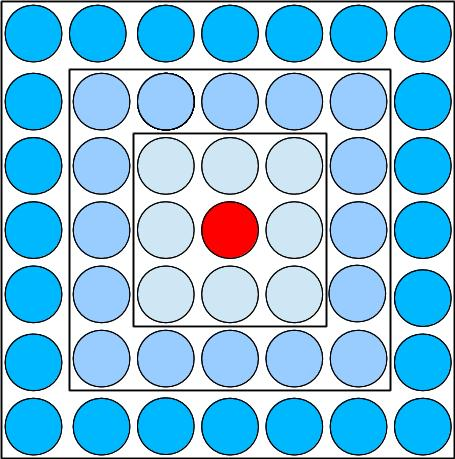
\includegraphics[width=0.2\linewidth]{img/parte2-vecindario.jpg}
					\caption{Función de vecindad.}
				\end{figure}
			\item REGLA DE KOHONEN: Actualización de los $W_{i}$.
					\begin{align*}
					 W_{i}(t+1) &=  \begin{cases}
										W_{i}(t) + \alpha(t) [ \varepsilon(t) - W_{i}(t) ] & i \in N_{c} \\
										W_{i}(t)                                           & i \not \in N_{c}  
									\end{cases} \\
					\end{align*}
			\item $\eta(t)$ es el coeficiente de aprendizaje dinámico, decreciente en el tiempo.
				\begin{align*}
					\Delta W_{ij} = \alpha(t) [ \varepsilon(t) - W_{i}(t) ]
					\alpha(t) = \eta \lambda(i,c)
					\lambda(i,c) = {\rm e}^x 
				\end{align*}
		\end{itemize}
\end{itemize}
 


\begin{figure}[ht!]
	\centering
	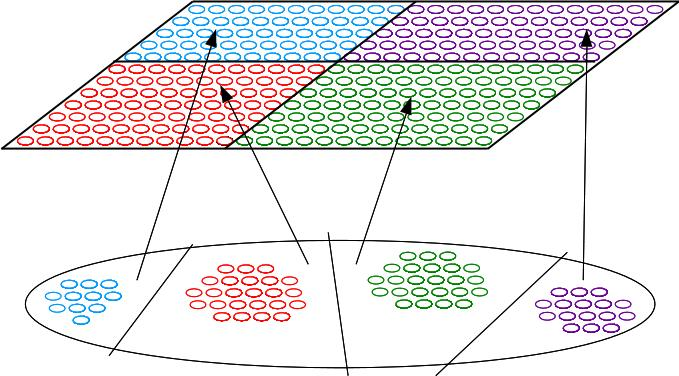
\includegraphics[width=0.7\linewidth]{img/kohonen4clases.jpg}
	\caption{Ejemplo con cuatro clases.}
\end{figure}

Para que un modelo sea auto-organizado debemos elegir el sigma $\sigma$ y  el eta $\eta$ adecuados. El sigma será utilizado como parámetro de la Gauseana y medirá la dispersión, cuantas 
neuronas vecinas a la neurona activada modificarán sus pesos. Por otro lado, el $\eta$ será el coeficiente de aprendizaje de nuestra red.

